
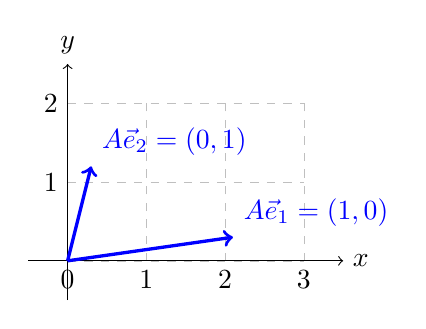
\begin{tikzpicture}
    \draw[step=1,help lines, dashed,lightgray] (0,0) grid (3,2);
    %draw axis value
    \foreach \x in {0,1,2,3}
        {%
            \draw (\x,0) -- (\x,0) node [below] {$\x$};
        }
    \foreach \y in {1,2}
        {%
            \draw (0,\y) -- (0,\y) node [left] {$\y$};
        }
    %draw lines
    \draw [->] (-0.5,0) -- (3.5,0) node[right]{$x$};
    \draw [->] (0,-0.5) -- (0,2.5) node[above]{$y$};
    \draw [->,blue,very thick] (0,0) -- (2.1,0.3) node[above right]{$\m{A}\vec{e}_1=(1,0)$};
    \draw [->,blue,very thick] (0,0) -- (0.3,1.2) node[above right]{$\m{A}\vec{e}_2=(0,1)$};
\end{tikzpicture}
\captionof{figure}{{\footnotesize $\m{A}\vec{e}$}}
\label{fig:matrix-and-matrix-operation-d1}
